%& -shell-escape
\documentclass[12pt, a4paper]{article}

\usepackage[hmargin=2.5cm, vmargin=2cm]{geometry}
\usepackage{amsthm, amssymb, mathtools, yhmath, graphicx}
\usepackage{fontspec, type1cm, titlesec, titling, fancyhdr, tabularx}
\usepackage{color}
\usepackage{unicode-math}
\usepackage{float}
\usepackage{hhline}
\usepackage{comment}
\usepackage[abbreviation,per-mode=symbol]{siunitx}
\usepackage{csvsimple}
\usepackage{subcaption}
\usepackage[CheckSingle, CJKmath]{xeCJK}
\usepackage{CJKulem}
\usepackage{enumitem}
\usepackage{tikz}
\usepackage[siunitx]{circuitikz}
\usepackage{wrapfig}
%\setCJKmainfont[BoldFont=cwTex Q Hei]{cwTex Q Ming}
%\setCJKsansfont[BoldFont=cwTex Q Hei]{cwTex Q Ming}
%\setCJKmonofont[BoldFont=cwTex Q Hei]{cwTex Q Ming}
\setCJKmainfont[BoldFont=cwTeX Q Hei]{cwTeX Q Ming}

\def\normalsize{\fontsize{12}{18}\selectfont}
\def\large{\fontsize{14}{21}\selectfont}
\def\Large{\fontsize{16}{24}\selectfont}
\def\LARGE{\fontsize{18}{27}\selectfont}
\def\huge{\fontsize{20}{30}\selectfont}

%\titleformat{\section}{\bf\Large}{\arabic{section}}{24pt}{}
%\titleformat{\subsection}{\large}{\arabic{subsection}.}{12pt}{}
%\titlespacing*{\subsection}{0pt}{0pt}{1.5ex}

\parindent=24pt

\DeclarePairedDelimiter{\abs}{\lvert}{\rvert}
\DeclarePairedDelimiter{\norm}{\lVert}{\rVert}
\DeclarePairedDelimiter{\inpd}{\langle}{\rangle}
\DeclarePairedDelimiter{\ceil}{\lceil}{\rceil}
\DeclarePairedDelimiter{\floor}{\lfloor}{\rfloor}

\newcommand{\unit}[1]{\:(\text{#1})}
\newcommand{\df}[1]{\mathop{}\!\mathrm{d^#1}}
\newcommand{\img}{\mathrm{i}}
\newcommand{\dD}{\mathrm{d}}
\newcommand{\dI}{\,\mathrm{d}}
\newcommand{\paral}{\mathbin{\|}}

\title{ \bf {\Huge 電子電路實驗6:Power Amplifiers}\\ 實驗結報}
\author{B02901178 江誠敏}

\begin{document}

\maketitle


\section{實驗結果}
\subsection{Class A output stage}
\begin{center}
	\begin{tabular}{p{3cm}p{4.5cm}}
	\hline
	項目 & 量測值 \\
  \hline
  \hline
  $V_{BB}$ & $\SI{840}\mV$ \\
  \hline
  \end{tabular}
\end{center}

\subsection{Class AB output stage}
\begin{center}
	\begin{tabular}{p{3cm}p{4.5cm}}
	\hline
	項目 & 量測值 \\
  \hline
  \hline
  $V_{CE3}$ & $\SI{841}\mV$ \\
  $V_{REN}$ & $\SI{920}\mV$ \\
  $V_{REP}$ & $\SI{550}\mV$ \\
  $R_b$ & $\SI{213}{\ohm}$ \\
  $V_{BB}$ & $\SI{200}\mV$ \\
  \hline
  \end{tabular}
\end{center}

\section{結報問題}

\begin{enumerate}[itemsep=20pt, topsep=10pt]

  \item {How to identify whether a power amplifier (PA) is class-B PA?} \\[10pt]
    答: 與 Class A amplifier 不同, Class B amplifier 只會導通半個周期,因此很容易
    從 $v_i\text{--}v_o$ Trasfer 圖上看出差異。(可用示波器的 $X\text{--}Y$ mode 觀察。)

    \begin{figure}[H]
      \centering
      \begin{subfigure}{0.45\textwidth}
        \centering
        \begin{tikzpicture}[domain=0:6, samples=100]
          \draw[very thin,color=gray] (-0.1,-1.1) grid (5.9,2.9);
          \draw[->] (-0.2,0) -- (6.2,0) node[right] {$v_i$};
          \draw[->] (0,-1.2) -- (0,3.2) node[above] {$v_o$};
          \draw[color=red, line width=0.3mm] plot[id=sin] function{sin(x*2)} ;
        \end{tikzpicture}
        \caption{Class A amplifier}
      \end{subfigure}
      \begin{subfigure}{0.45\textwidth}
        \centering
        \begin{tikzpicture}[domain=0:6, samples=100]
          \draw[very thin,color=gray] (-0.1,-1.1) grid (5.9,2.9);
          \draw[->] (-0.2,0) -- (6.2,0) node[right] {$v_i$};
          \draw[->] (0,-1.2) -- (0,3.2) node[above] {$v_o$};
          \draw[color=blue, line width=0.3mm] plot[id=sin] function{(sin(x*2)+abs(sin(x*2)))/2} ;
        \end{tikzpicture}
        \caption{Class B amplifier}
      \end{subfigure}
    \end{figure}

  \item {What is crossover distortion? What is the reason of occurring it? } \\[10pt]
    答: Crossover distortion 是因為 Class AB/B 的 BJT 只會導通半個周期,而在兩個互補的BJT
    的半周期間, BJT 的電壓會掉出 active 區間,使得電壓有偏誤產生,即為 crossover distortion.
    從 $v_i\text{--}v_o$ Trasfer 圖上看出差異。(可用示波器的 $X\text{--}Y$ mode 觀察。)
    \begin{figure}[H]
      \centering
      \begin{tikzpicture}[]
        \draw[very thin,color=gray] (-3.0,-2.9) grid (3.0,2.9);
        \draw[->] (-3.2,0) -- (3.2,0) node[right] {$v_i$};
        \draw[->] (0,-2.9) -- (0,2.9) node[above] {$v_o$};
        \draw[color=red, line width=0.3mm] plot[id=sin,domain=-3:3,samples=100] function{3*sin(x)*(1-exp(-0.5*x*x))} ;
        \draw[color=blue, line width=0.4mm] plot[id=sin,domain=-0.5:0.5,samples=100] function{3*sin(x)*(1-exp(-0.5*x*x))} ;
      \end{tikzpicture}
      \caption{Example of crossover distortion.}
    \end{figure}


  \item {Try to explain how to calculate the power transfer efficiency of class-B PA? } \\[10pt]
    答: 可在電源供應器和 load 都同時接上伏特計和安倍計,假設電源供應器的讀值分別為 $V_S, I_S$, load 的
    讀值為 $V_L, I_L$ (接用 rms 計算),則 
    \[ \text{\%power transfer efficiency }  \approx \frac{V_L I_L}{V_S I_S} \cdot 100\% \] 

  \item {Does the crossover distortion exist in class-AB PA? Try to answer the 
       power transfer efficiency of class-AB PA is between which two kinds of 
     power amplifiers. } \\[10pt]
  答: Crossover distortion still exist in class-AB PA, but slightly smaller than class-B PA,
  which could be seen by the result of the experiment. \\
  The transfer efficiency of class-AB PA is between class-B and class-A. i.e,
  \[
    \text{class-A } < \text{ class-AB } < \text{ class-B}
  \]

\item {Please perform the simulation of the class-B power amplifier circuit shown 
    in Fig. 1. Determine what the transfer curve of $V_O\text{--}V_i$ is. 
    What is the $V_O\text{--}I_O$ curve if applying a sine wave signal with $\SI{10}\V$ amplitude,
  $\SI{0}\V$ the dc offset value, and $\SI{1}{\kilo\hertz}$ frequency in the input terminal?} \\[10pt]
    答: 這裡使用 Ngspice 模擬。我一開始使用實驗用的 MJE2955T, MJE3055T 來模擬,但是結果非常奇怪。
    \begin{figure}[H]
    \centering
      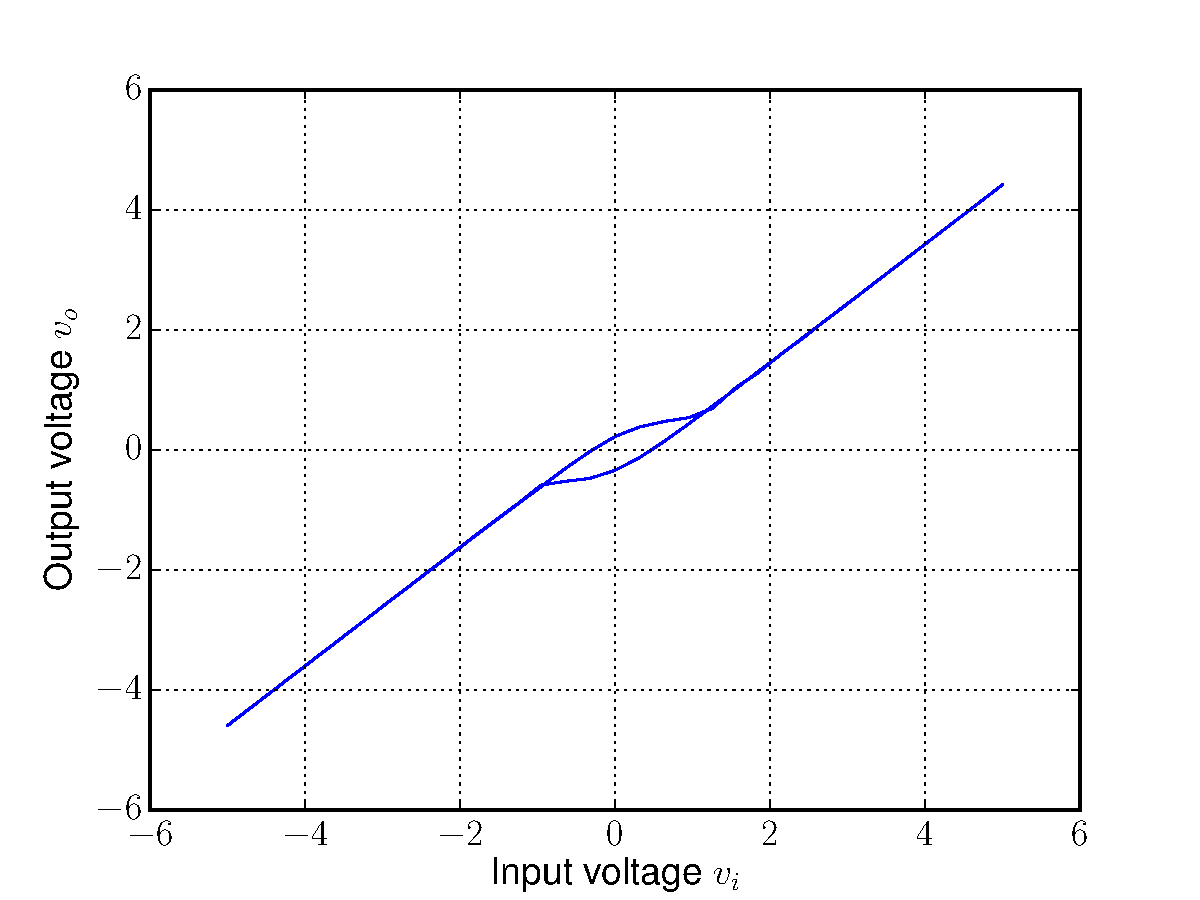
\includegraphics[width=.5\textwidth]{ngspice/p1vvbad.pdf}
    \caption{Simulation with MJEs}
    \label{fig:}
    \end{figure}
    可能是網路上提供的參數有點問題,但我也找不到其他免費的,因此改用 2N2222, 2N4032 來模擬。
    \begin{figure}[H]
      \begin{subfigure}{0.48\textwidth}
        \centering
        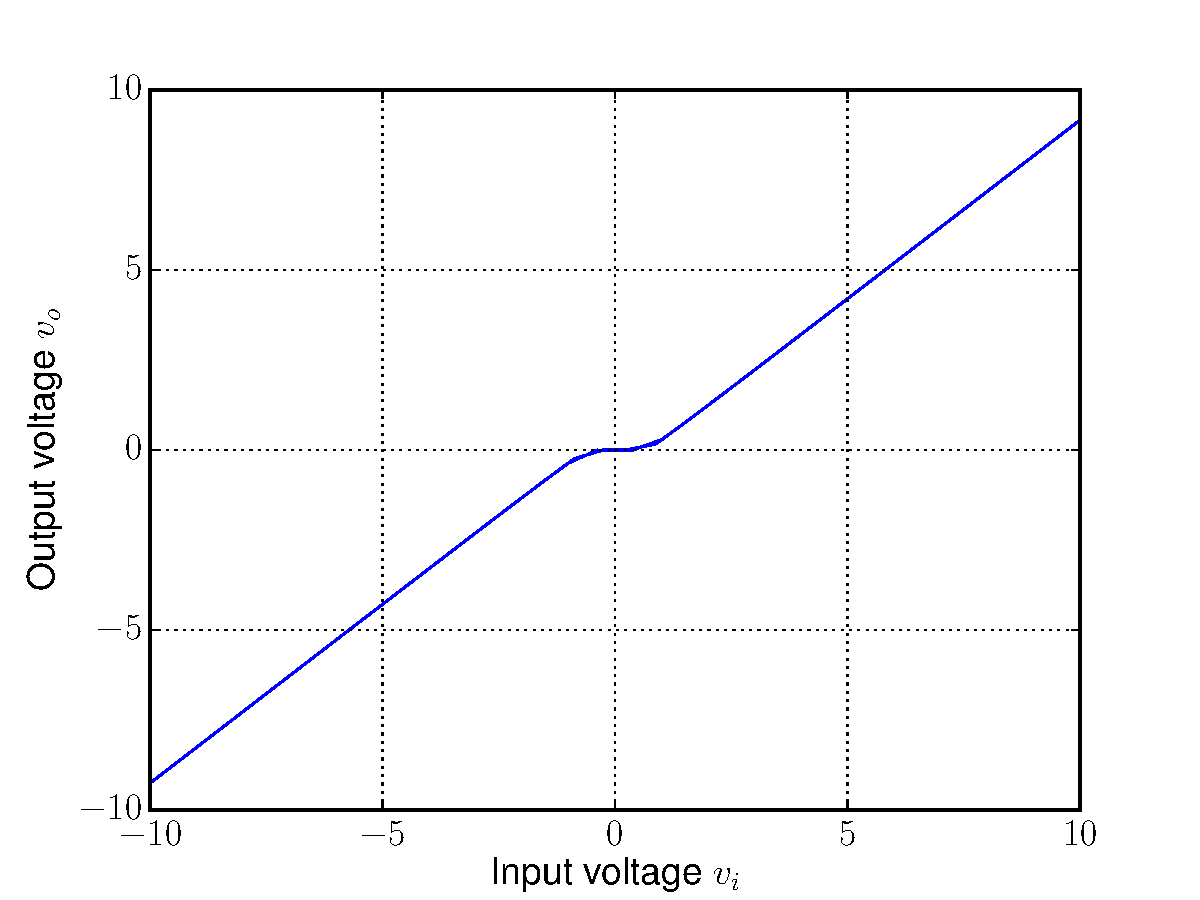
\includegraphics[width=\textwidth]{ngspice/p1vv.pdf}
        \caption{$V_O\text{--}v_i$ curve.}
      \end{subfigure}%
      \begin{subfigure}{0.48\textwidth}
        \centering
        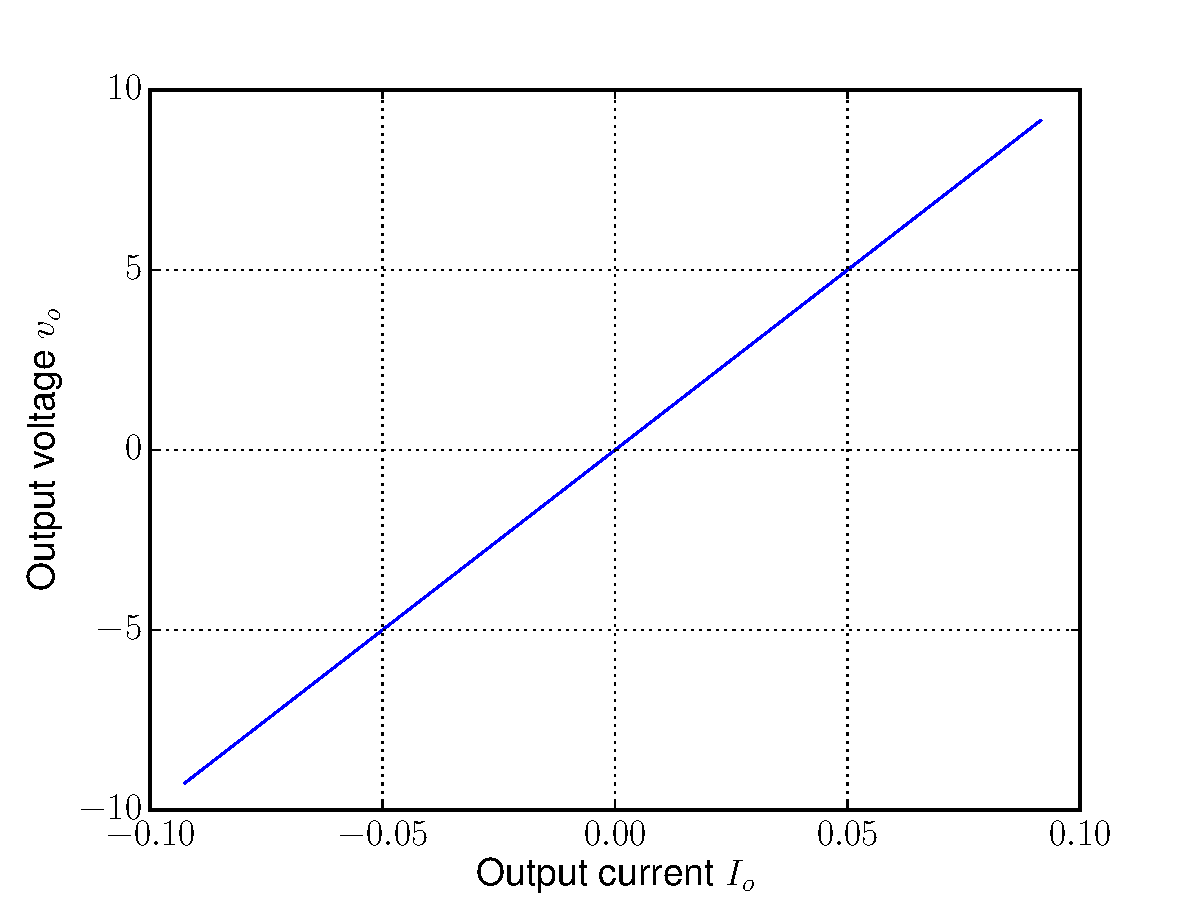
\includegraphics[width=\textwidth]{ngspice/p1iv.pdf}
        \caption{$V_O\text{--}I_O$ curve.}
      \end{subfigure}
    \caption{Simulation with 2N*}
    \end{figure}
\item {In Fig. 8, please perform the simulation of the class-B power amplifier circuit.
    Determine what the transfer curve of $V_O\text{--}V_i$ is. What is the $V_O\text{--}I_O$ curve 
    if applying a sine wave signal with $\SI{10}\V$ amplitude, $\SI{0}\V$ DC-offset value,
  and $\SI{1}{\kilo\hertz}$ frequency in the input terminal? } \\[10pt]
    答: 在這個電路中, $Q_3, Q_4$ 提供了一個穩定的電壓差,把 crossover distortion 給抵消掉,因此只要
    $I_{\text{bias}}$ 不要太小(如下圖) ,維持 BJT 在 active mode 即可!
    \begin{figure}[H]
    \centering
      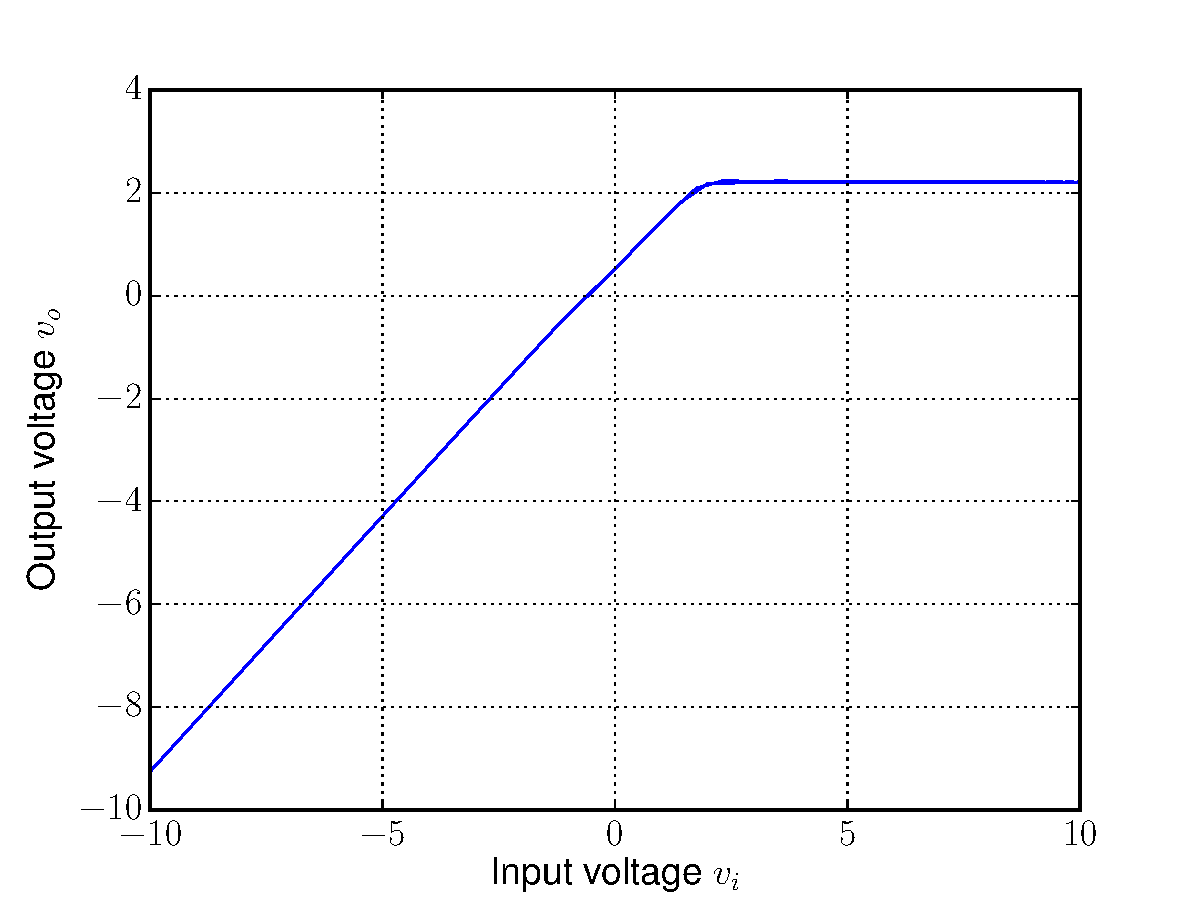
\includegraphics[width=.5\textwidth]{ngspice/p2vvbad.pdf}
      \caption{$I_{\text{bias}} = \SI{10}{\micro\ampere}$}
    \label{fig:}
    \end{figure}
    以下是 $I_{\text{bias}} = \SI{10}\mA$ 的模擬結果。
    \begin{figure}[H]
      \begin{subfigure}{0.48\textwidth}
        \centering
        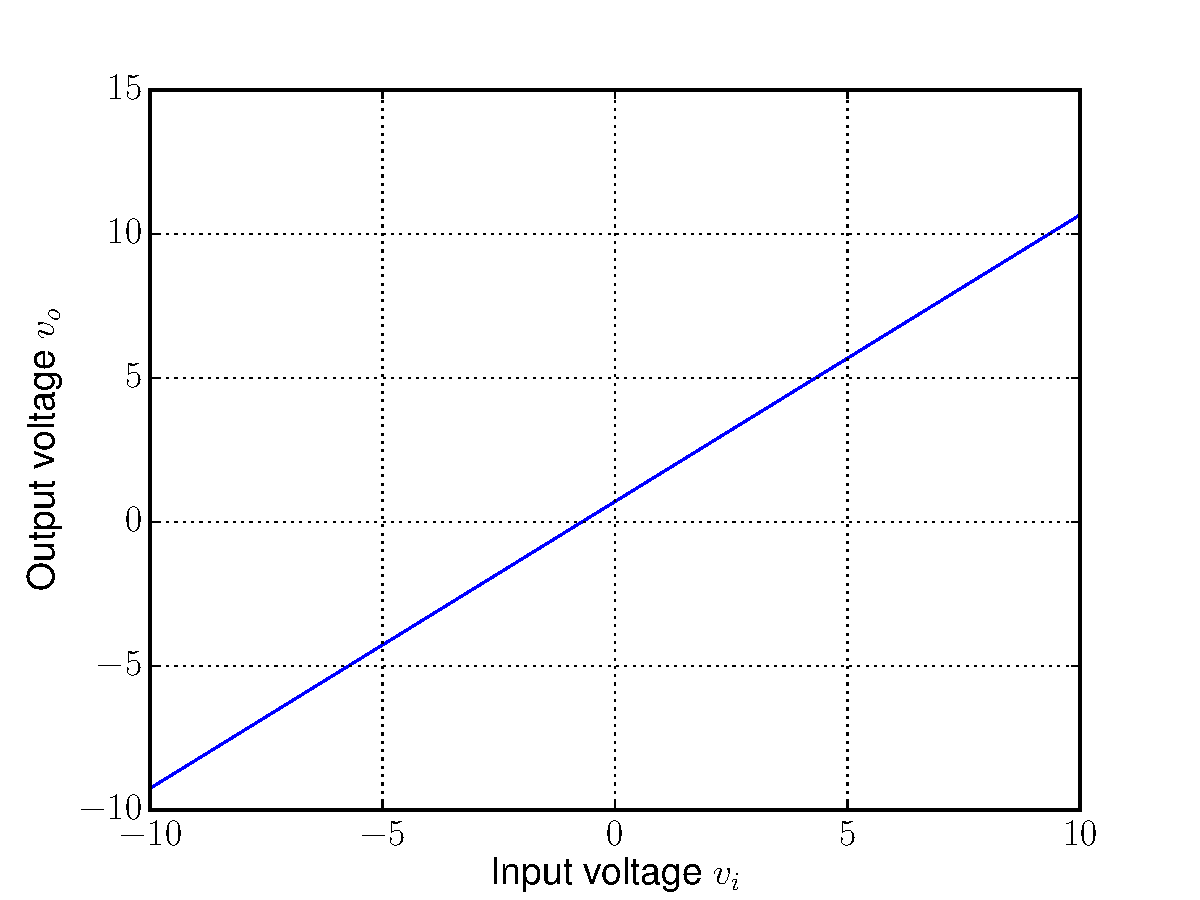
\includegraphics[width=\textwidth]{ngspice/p2vv.pdf}
        \caption{$V_O\text{--}v_i$ curve.}
      \end{subfigure}%
      \begin{subfigure}{0.48\textwidth}
        \centering
        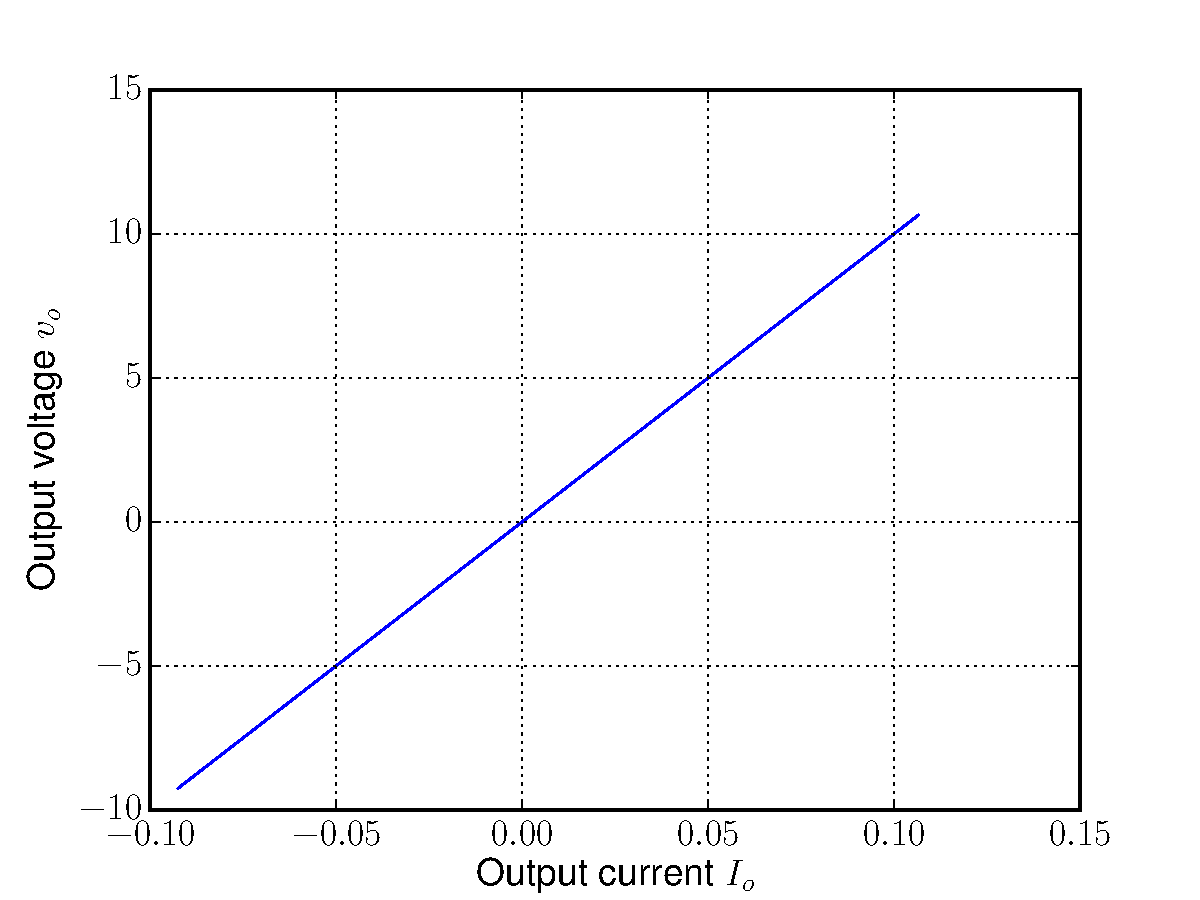
\includegraphics[width=\textwidth]{ngspice/p2iv.pdf}
        \caption{$V_O\text{--}I_O$ curve.}
      \end{subfigure}
    \caption{Simulation with 2N*}
    \end{figure}
    這兩題 $V_O\text{--}I_O$ 似乎顯然是一條斜率為 $R_L$ 的直線。
  \item {請設計一個電路,使得BJT的 $\beta$ 值可以被量測到。} \\[10pt]
    答: 可利用 BJT 在 active mode 時, $I_C / I_B  = \beta$ ,因此我們只要給
    $V_{BE}$ 一個適當的跨壓 ($\approx \SI{0.7}\V$) ,在量測 $I_C, I_B$ 的比值
    即可!
    \begin{figure}[H]
      \centering
        \begin{tikzpicture}[american voltages, scale=1.25]
          \draw[color=black, thick]
          (0, 0) node[ground]{} to[short] (0, 1) node[npn, anchor=E](q1){}
          (q1.B) to[ammeter,mirror,l=$I_B$] ++(-1.5, 0) to[V=$V_{BE}$] ++(0, -1.5) node[ground]{}
          (q1.C) to[ammeter, l=$I_C$] ++(1.5, 0) to[R] ++(0, -2.25) node[ground]{}
          ;
        \end{tikzpicture}
    \end{figure}
\end{enumerate}

\section{心得}
今天的實驗雖然複複雜雜,但是只要耐心做,其實好像沒那麼困難。 我想應該是因為這
次做的是比較「大訊號」的東西,儀器在這部分比較不會出問題,如果是小訊號的話,
你就要開始擔心示波器的雜訊、線路接觸不良等等麻煩的問題。 真希望以後都不要在
做跟小訊號相關的東西了!
\end{document}

